% KEMField documentation for the Kassiopeia Guide

\section{Comprehensive Field Simulation: KEMField}\label{sec:KEMField}

\subsection{Electrostatic Solver: The RobinHood Method}

The Robin Hood method was developed by Predrag Lazic,  Hrvoje Stefancic, and Hrvoje Abraham~\cite{RH1,RH2} and the reader is encouraged to read the cited literature.  At its core, Robin Hood is a matrix inversion algorithm but, as such, it is particularly suited for electrostatic problems, especially those whose boundary conditions are well-defined. Let us first define the problem to be solved, and then discuss the implementation of Robin Hood toward its solution.

Consider the case where one wishes to know the potential, $U(\vec{x})$ at some point in space ($\vec{x}$).  To find the potential, one needs to calculate the contribution from each charge sub-element (with charge density $\sigma_i$) which contributes to the potential.  

\begin{equation}
U(\vec{x}) = \int_{\partial V} G(\vec{x},\vec{x'}) \sigma(\vec{x}') dS'
\end{equation}

\noindent Here, the integration is carried over some surface $dS'$ with a charge density $\sigma$ at a location $\vec{x}'$.  Green's function, $G(\vec{x},\vec{x'})$ is given by the expression

\begin{equation}
G(\vec{x},\vec{x'}) =  \frac{1}{4 \pi \epsilon_0} \frac{1}{|\vec{x}-\vec{x}'|}
\end{equation}

With discretization, one imposes the assumption that the surface charge density is constant across $dS'$.  The integration therefore reduces to a sum

\begin{equation}
U_i = \sum_{j=1}^N I_{ij} \sigma_j
\label{eq:potential}
\end{equation}

\noindent where $U_i$ is the potential of the sub-element $i$, $\sigma_j$ is the charge density of sub-element $j$ of $N$ and $I_{ij}$ is given by...

\begin{equation}
I_{ij} = \frac{1}{4\pi\epsilon_0}\int_{\Delta S_j} \frac{dS_j}{|\vec{r}_i - \vec{r}_j|} 
\end{equation}

In the case where one is dealing with only metal conductors, all such charges reside at the surfaces.  Furthermore, all metal surfaces are at {\em equipotential} (either defined by the configuration of the experiment or by the electrostatic configuration itself).  This essentially sets up the necessary boundary conditions one needs to solve.  The charge densities $\sigma_i$ will arrange themselves until all the surfaces in the problem are indeed at equipotential.  Once the charge configuration is known, then the potential everywhere in space (not just at the surfaces) can be known as well\footnote{This last condition is guaranteed by the nature of Laplace's equation.}.  

Boundary element methods are directed at solving the above matrix, and the Robin Hood method is no exception.  At its heart, it is a variation of the boundary element method.  However, it appears to be {\em the most efficient} implementation of BEM, both in terms of computation time and memory use.  

\subsubsection{Implementation with Conductors in Isolation}

To describe the algorithm, consider the following simple example.  An isolated metal cube has a total charge $Q$ distributed over its surface.  We subdivide the surface into smaller sub-elements (typically rectangles and/or triangles, though this is not necessary), each with a small amount of charge $q$ over each of their surfaces.  The initial assignment of charges can be random since we do not know the proper configuration at this stage.  Using this (incorrect) charge configuration, we can therefore compute the potential at each sub-element using Eq.~\ref{eq:potential}.  Of course, the potential across the surface at this point will {\em not} be an equipotential because the charge configuration is incorrect.

To correct the charge configuration, we select two sub-elements from the configuration ($m$ and $n$).  The sub-elements are selected such that they are furtherest away from the average potential.  We then {\em redistribute} the charges such that they are both at the same potential.  For the case of two sub-elements, there is an exact solution to the amount of charge that needs to be moved from one element to the other.

\begin{equation}
\delta \sigma = \frac{U_m - U_n}{I_{mm} + I_{nn} - I_{mn} - I_{nm}}
\end{equation}

\noindent where $U_{m,n}$ is the potential at the two selected points. The new potential due to this redistribution is given by

\begin{eqnarray}
U_m' = U_m - I_{mm}\delta \sigma + I_{mn}\delta \sigma\\
U_n' = U_n + I_{nn}\delta \sigma - I_{nm}\delta \sigma
\end{eqnarray}

The charge exchange of $\delta \sigma$ has two effects. First, it now forces $U_m'$ and $U_n'$ to be at the same potential and secondly, these new charges propagate their effects to their neighboring elements.  This allows the solution to quickly converge.  The process is then repeated until the maximum difference between the equipotential solution and $U_i$ falls below some pre-determined user-defined threshold.

\subsubsection{Implementation with Conductors at a Defined Potential}

As another example, let us consider now the case where the cube is held at a fixed potential $U_0$.  The algorithm is very similar to the case of the isolated cube, except one can relax the charge conservation condition (because effectively one can extract the charge from an external source).  Again, one initially randomizes the charge distribution and then selects two elements whose potential is furthest away from the equipotential $U_0$.  The amount of charge added to the two selected elements ($k$ and $l$) is given by the following expression:

\begin{eqnarray}
\delta \sigma_k = \frac{(U_0 - U_k)I_{ll} - (U_0-U_l)I_{kl}}{I_{kk} I_{ll} -I_{kl}I_{lk}}\\
\delta \sigma_l = \frac{(U_0 - U_l)I_{kk} - (U_0-U_k)I_{kl}}{I_{kk} I_{ll} -I_{kl}I_{lk}}
\end{eqnarray}

The adjusted potential is given by 

\begin{eqnarray}
\label{eq:charge_exchange}
U_k' = U_k + I_{kk} \delta \sigma_k + I_{kl} \delta \sigma_l \\
U_l' = U_l + I_{ll} \delta \sigma_l + I_{kl} \delta \sigma_k
\end{eqnarray}

The solution quickly converges, as the added charges equalize not just the selected elements, but its nearest neighbors as well.

\subsubsection{Charge Exchange Generalization}

For both the insulated and non-insulated conductors, we have shown the solution for the case when two electrodes exchange/add/subtract charges.  We can generalize the solution to the case of M electrodes exchanging charge, where $1 \le M \le N$.  For the case of electrodes held at fixed potential, this is equivalent to the inversion of a $M \times M$ matrix:

\begin{equation}
\sum_{j = 1}^{M} I_{ij} \sigma_j = U_i
\end{equation}

\noindent where $I_{ij}$ is the $M \times M$ Coulomb matrix as defined previously.  Both indexes $i$ and $j$ range from 1 to $M$. Note that for M=2, one reproduces Eq.~\ref{eq:charge_exchange}.

The same generalization can be made for the insulated charge case.  Here, one must explicitly introduce the conservation of charge as part of the matrix to be solved.   In general, one can impose the conservation of charge as follows:

\begin{equation}
\sum_{j=1}^{M} \sigma_j = 0
\end{equation}

As for the condition imposed by the equipotential surface, one realizes that all the potentials at each altered electrode are identical.  One way to write this condition is as follows:

\begin{equation}
\sum_{j=1}^{M}(I_{i,j} - I_{i+1,j}) \sigma_j = U_{i+1}-U_i
\end{equation}

Note that index $i$ ranges only from 1 to $M-1$.  The combination of the two constraints produces an $M \times M$ matrix equation which can be inverted to solve for $\sigma_j$.  Note that for the isolated conductor, $M > 1$.

\subsubsection{Advantages and Caviats}

The Robin Hood method is very effective in computing the charge configuration within the context of computing algorithms for a number of reasons, some of which are iterated below:

\begin{itemize}
\item The algorithm searches for the maximum deviation from equipotential for each sub-element.  As such, it can readily make use of functions such as MAX/MIN, which are extremely efficient for arrays.  Furthermore, since it corrects elements which are furthest away from the solution (and those elements affect those around them, due to the properties of Green's function), there is rapid convergence of all charges.
\item In implementing the charge correction, it is most advantageous to recompute the elements $I_{ij}$.  In doing so, there is no need to create a large array.  As such, the memory allocation grows as $N$ rather than $N^2$.  Direct matrix inversion techniques require either $N^2$ or, in the most effective implementation of these systems, $N \log{(N)}$.
\item Since the algorithm is step-oriented, it can be very effectively be distributed to multiple processors.  Therefore, implementation on parallel systems (such as MPI) is straightforward.
\end{itemize}

In the next section, we will discuss the speed and accuracy of this algorithm.  In order to ensure convergence, the user needs to keep in mind that the matrix must possess the following properties:

\begin{itemize}
\item  {\it Diagonal Dominant:}  The algorithm converges only if the matrix being solved is diagonally dominant.  This condition is guaranteed due to the nature of Green's function for electro- and magneto- statics~\cite{Gluck}.
\item  {\it Linearity:}  This condition is guaranteed due to the nature of Maxwell's equation.
\item  {\it Uniqueness:}  If two or more elements are defined but their centers overlap, the solution is infinite and the solution quickly diverges.  In fact, RH by virtue of this property can quickly discover if elements overlap.  Note that this latter condition is a problem with BEM methods as well.
\end{itemize}

\subsubsection{Verification}

The Robin Hood algorithm has been successful implemented in KATRIN's Kassiopeia Monte Carlo framework, within the context of KEMField.  Its implementation is similar to BEM in that the electrode properties need to be defined prior to solving for the charge distribution.  The algorithm has been adapted for both single and parallel processing (MPI), though the majority of the tests described have been executed on a single processor (Mac OS X 10.6.4, 2.53 GHz Intel Core 2 Duo processor).  Since RH is most effective as a 3D discrete solver, we typically discretize the surfaces of our test electrodes into rectangles and triangles, though any electrode surface geometry can be used.  RH can be implemented to stop when a certain accuracy is reached or a certain number of iterations are processed.  The accuracy is computed using the formula

\begin{equation}
\epsilon = \frac{\sqrt{\frac{1}{N}\sum_i^N (U_i - U_0)^2}}{U_0}
\end{equation}

\noindent where $U_i$ is the potential at electrode $i$ and $U_0$ is the fixed potential at surface.  For these initial tests, we stop the iteration whenever $\epsilon < 10^{-15}$ or the number of iterations exceeds 200,000.

\subsection{Unit Cube}

Our first test has been conducted on a unit cube.  The capacitance of a unit cube in normalized units ($1/4\pi\epsilon_0$) is $0.66067786 \pm 8 \times 10^{-8}$\cite{RH2}\footnote{Incidentally, the most accurate calculation of the cube capacitance was achieved using the RH method (see citation).}.  The cube is discretized in a number of triangles and electrodes and the charge is then computed assuming the potential is held fixed at 1 V.  Table~\ref{tab:cube} shows the results using RH.

\begin{figure}[htbp]
\begin{center}
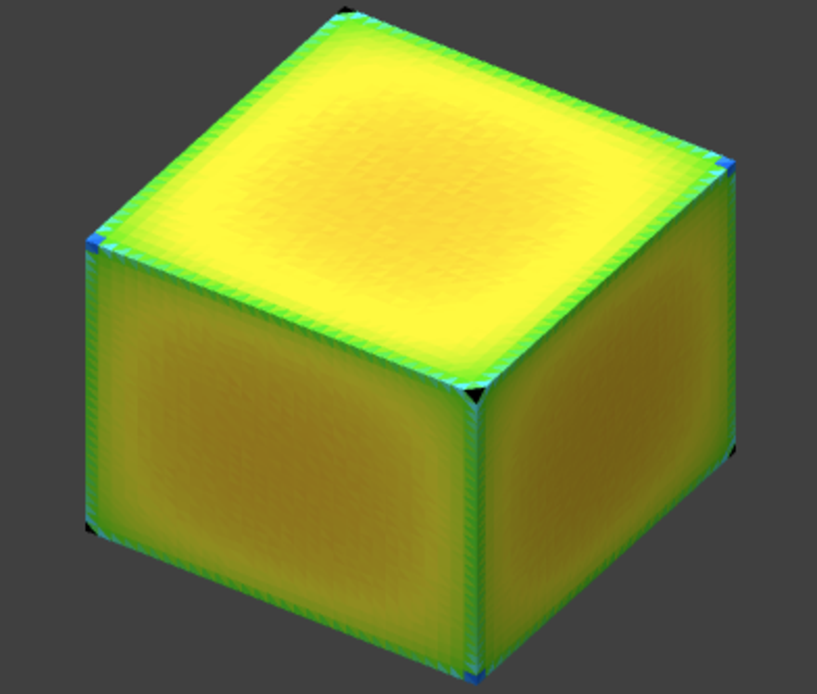
\includegraphics[width=0.6\textwidth]{images/KEMFieldPlots/cube_pic.pdf}
\caption{Charge distribution on discrete cube held at fixed potential.}
\label{fig:thecube}
\end{center}
\end{figure}

\begin{table}[htdp]
\caption{Unit capacitance of a cube as calculated by Robin Hood using $N$ electrodes.  Accuracy reports on the percentage difference to a previously calculated cube capacitance.  All sub-elements are the same size (no refinement near edges), except where indicated.}
\begin{center}
\begin{tabular}{|c|c|c|c|c|}
\hline
Test No. & Number of Elements & Accuracy & Scaling & Number of Iterations \\
\hline
1 & 660 & 0.23\% & fixed & 8000 \\ 
2 & 2520 & 0.13\% & fixed & 30,000 \\
3 & 10,800 & 0.08\% & fixed & 50,000 \\
4 & 15,300 & 0.04\% & fixed & 190,000 \\
5 & 60,600 & 0.01\% & fixed & 200,000 \\
6 & 19,200 & 0.0046\% & variable & 30,000 \\
\hline
\end{tabular}
\end{center}
\label{tab:cube}
\end{table}%

For test cases 1 and 2, we also computed the capacitance using a more standard Boundary Element Method.  In each case, the results were identical.  Running test cases 3-6 on a single processor using BEM is extremely time consuming and was therefore abandoned.  In general, changing the length scale as one approaches the edge of the cube increases the convergence and accuracy of the results (for example, case 6 took 20 minutes to converge with an accuracy on the capacitance of better than $5\times10^{-5}$). Similar tests were conducted making use of MPI.  Results of these tests are shown in Figure~\ref{fig:cube_results}.

\begin{figure}[htbp]
\begin{center}
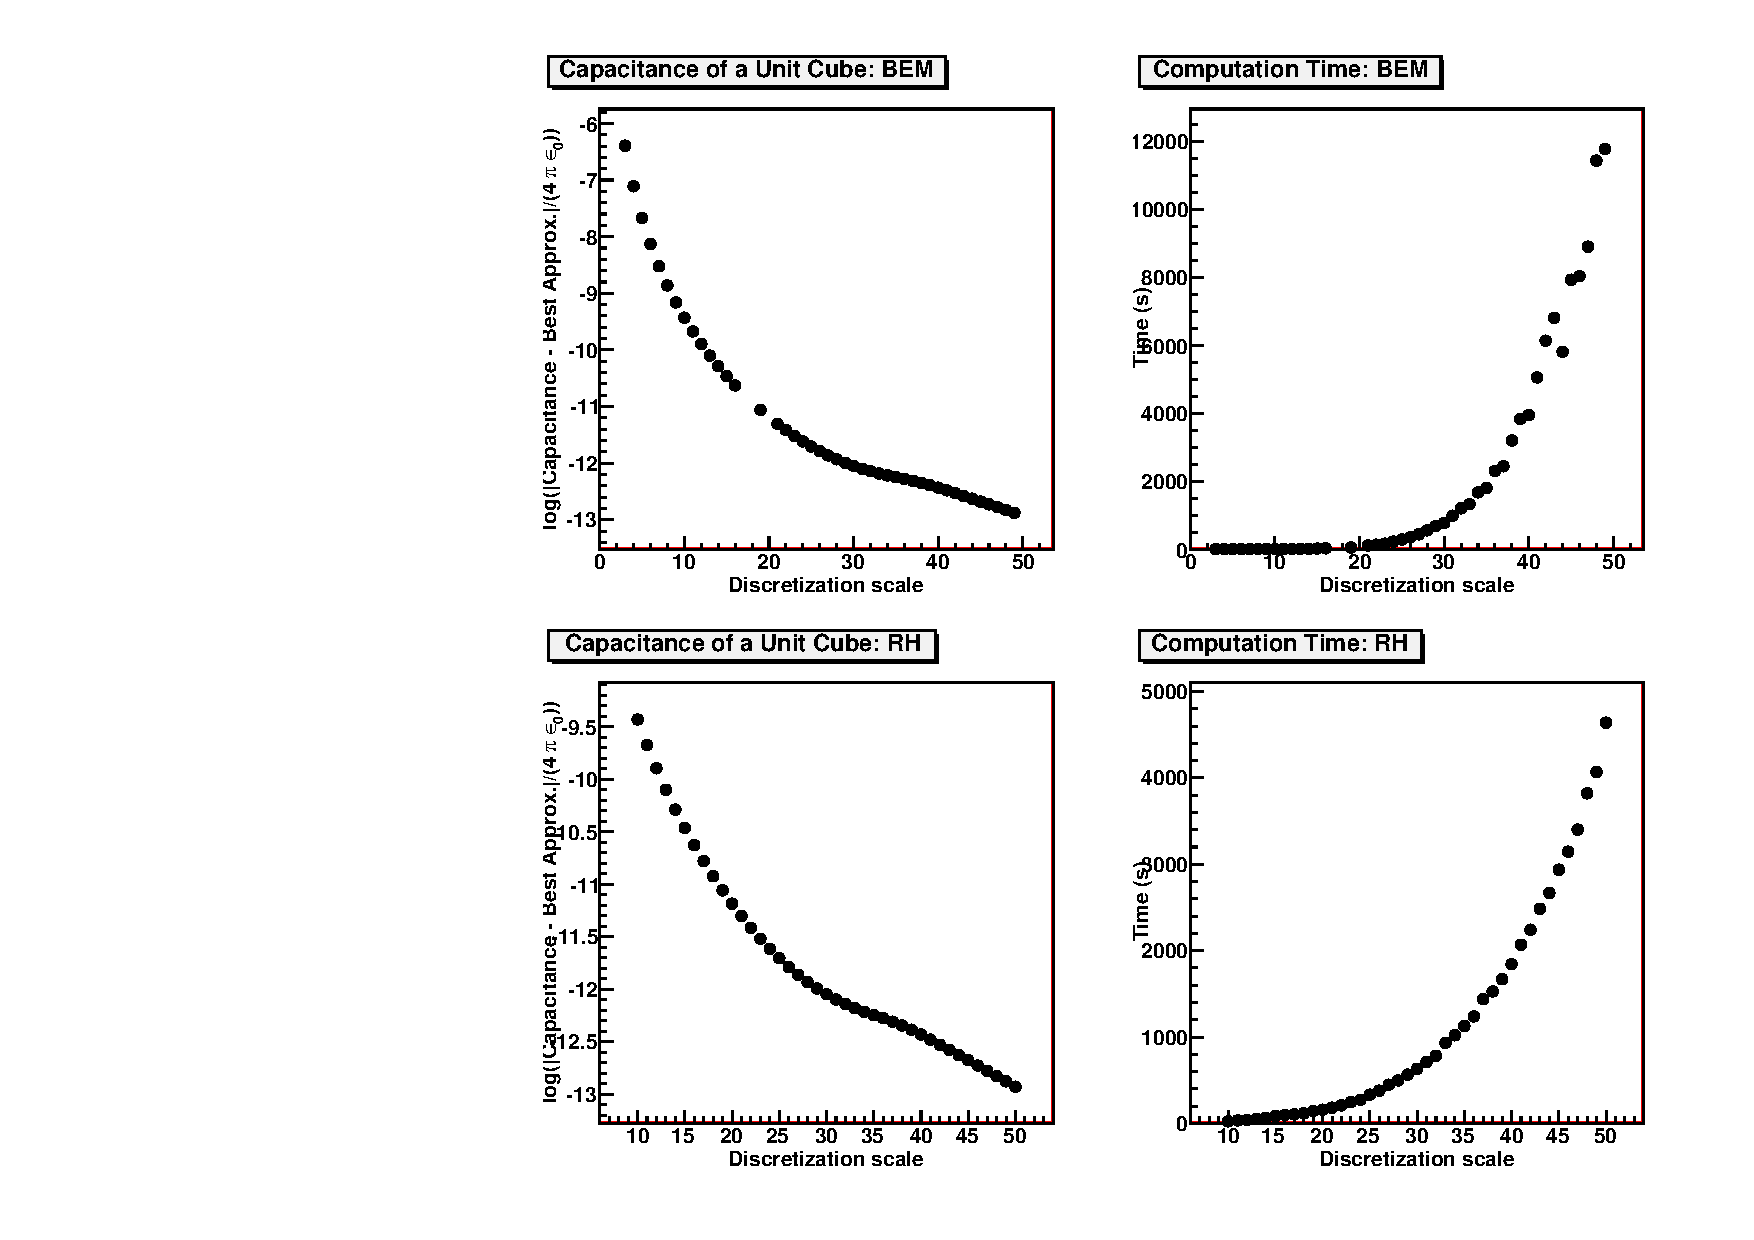
\includegraphics[width=\textwidth]{images/KEMFieldPlots/RH_vs_BEM.pdf}
\caption{Plot of accuracy and computation time for RH and BEM methods as a function of electrode discretization for a unit cube.}
\label{fig:cube_results}
\end{center}
\end{figure}

It is possible to fit the dependance of the accuracy (at least for the unit cube) as a function of iteration.  The following expression...

\begin{equation}
\epsilon \simeq \frac{A}{\sqrt{N}} e^{-\frac{n \tau}{N}}
\end{equation}

\noindent works very well.  Here, $n$ is the iteration number, $N$ is the number of electrodes, and $A$ and $\tau$ are constants.  In the case of the unit cube, $A\simeq 4$ and $\tau \simeq 2.4$, and are fairly independent of the number of electrodes used.  Note that if one assumes that the amount of time ($t$) to compute $n$ iterations depends linearly on $N$ as $t = n N \tau_0$, then one finds...

\begin{equation}
\epsilon \simeq \frac{A}{\sqrt{N}} e^{-\alpha \frac{t}{N^2}}
\end{equation}

\noindent where $\alpha = \frac{\tau}{\tau_0}$ is just a (processor-dependent) constant.  This is consistent with the observation by~\cite{RH1,RH2} that the computation time scales as $N^{1.35}$ for small $N$ and as $N^2$ for large $N$.  The memory footprint however, is always proportional to $N$.

Tests have also been performed on a unit disk with similar convergence behavior.

\subsection{M-Dependence}

The dependence of the convergence on the size of the swap matrix (in this notation, $M$) has also been tested.  The results are shown in Table~\ref{tab:M}.  In general the convergence is best for $M=1$ and gets worse for $M>1$.  Note that $M>1$ for isolated charge cases.

\begin{table}[htdp]
\caption{The convergence dependence on the number of charge exchange electrodes $(M)$ for a test electrode system.  $N$ refers to the total number of electrodes, $n$ is the number of iterations, $t$ is the computation time, and $\epsilon$ is the convergence metric.  In general, the total number of iterations for $M=1$ is greater than $M=2$, but the accuracy is better (for fixed computation time).}
\begin{center}
\begin{tabular}{|c|c|c|c|c|}
\hline
Electrodes & M & Iterations & $\epsilon$ & Time (s) \\ 
\hline
1800 & 1 & 10000 & $5.7 \times 10^{-4}$ & 60 \\
1800 & 2 & 5000 & $1.65 \times 10^{-3}$ & 60 \\
1800 & 6 & 1700 & $9.73\times 10^{-3}$ & 120 \\
\hline
4000 & 1 & 20000 & $1.8 \times 10^{-3}$ & 240 \\
4000 & 2 & 10000 & $2.9 \times 10^{-3}$ & 240 \\
\hline
7200 & 1 & 20000 & $2\times 10^{-1}$ & 360 \\
7200 & 2 & 10000 & $3 \times 10^{-1}$ & 360 \\
\hline
14000 & 1 & 100000 & $9\times 10^{-6}$ & 3600 \\
14000 & 2 & 50000 & $2 \times 10^{-5}$ & 3600 \\
\hline
28000 & 1 & 200000 & $9\times 10^{-6}$ & 21600 \\
28000 & 2 & 100000 & $2 \times 10^{-5}$ & 21600 \\
\hline
\end{tabular}
\end{center}
\label{tab:M}
\end{table}%


\subsubsection{Nested Spheres}

RH has also been tested using two nested metal spheres where the inner sphere held at 10 V while the outer sphere is held at ground (see Fig.~\ref{fig:nested_spheres}).  Gauss' law guarantees that inside the innermost sphere the potential everywhere should be constant (10 V).  Figure~\ref{fig:ns_results} shows the potential sampled from 50,000 points inside the innermost sphere for an accuracy $\epsilon$ of $10^{-1}$ and $10^{-4}$.  Note that the system quickly converges to the correct solution as the requirement on $\epsilon$ is tightened.

\begin{figure}[htbp]
\begin{center}
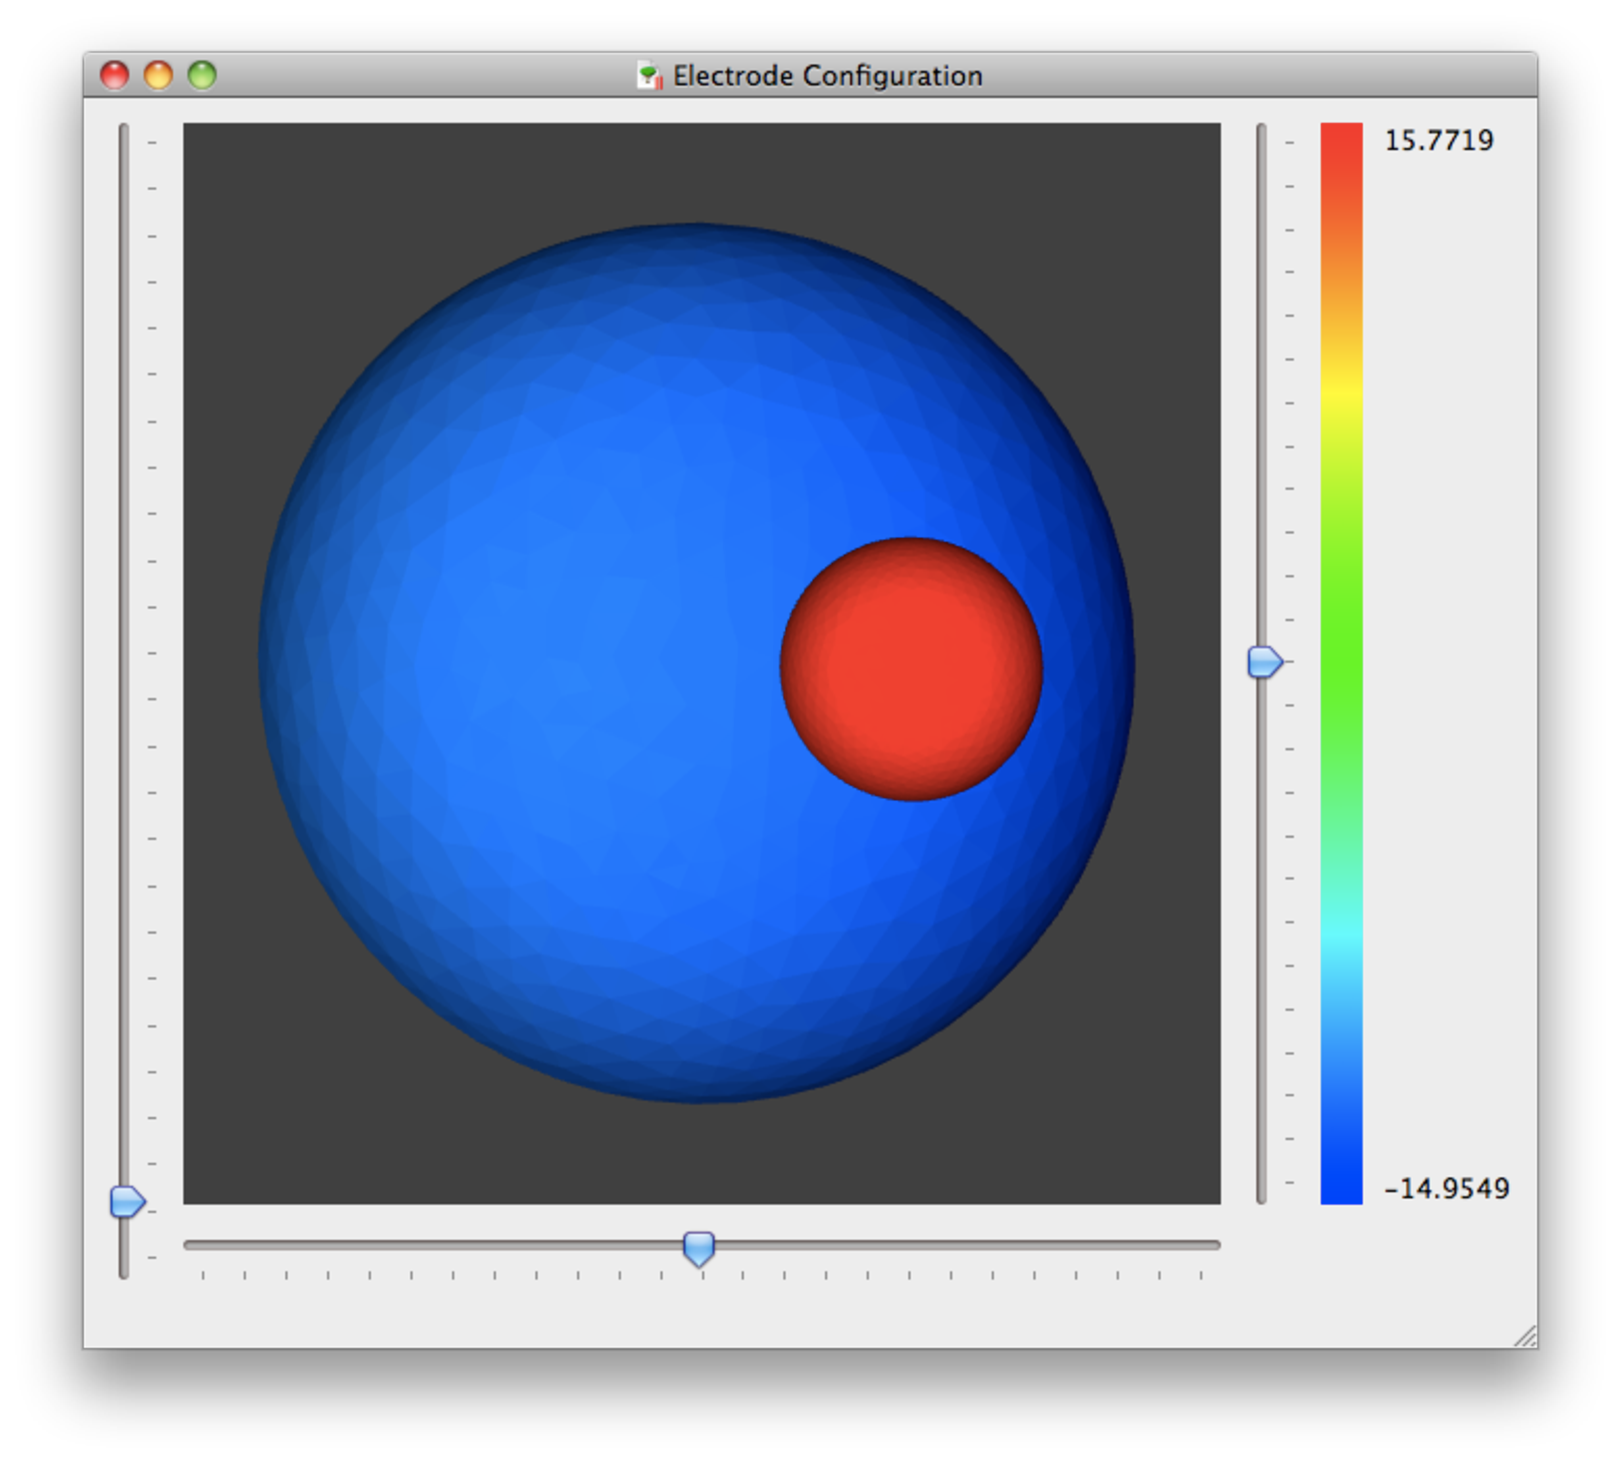
\includegraphics[width=\textwidth]{images/KEMFieldPlots/nestedSpheres.pdf}
\caption{Charge distribution calculated from two nested spheres held at two different potentials.}
\label{fig:nested_spheres}
\end{center}
\end{figure}

\begin{figure}[htbp]
\begin{center}
\begin{tabular}{c c}
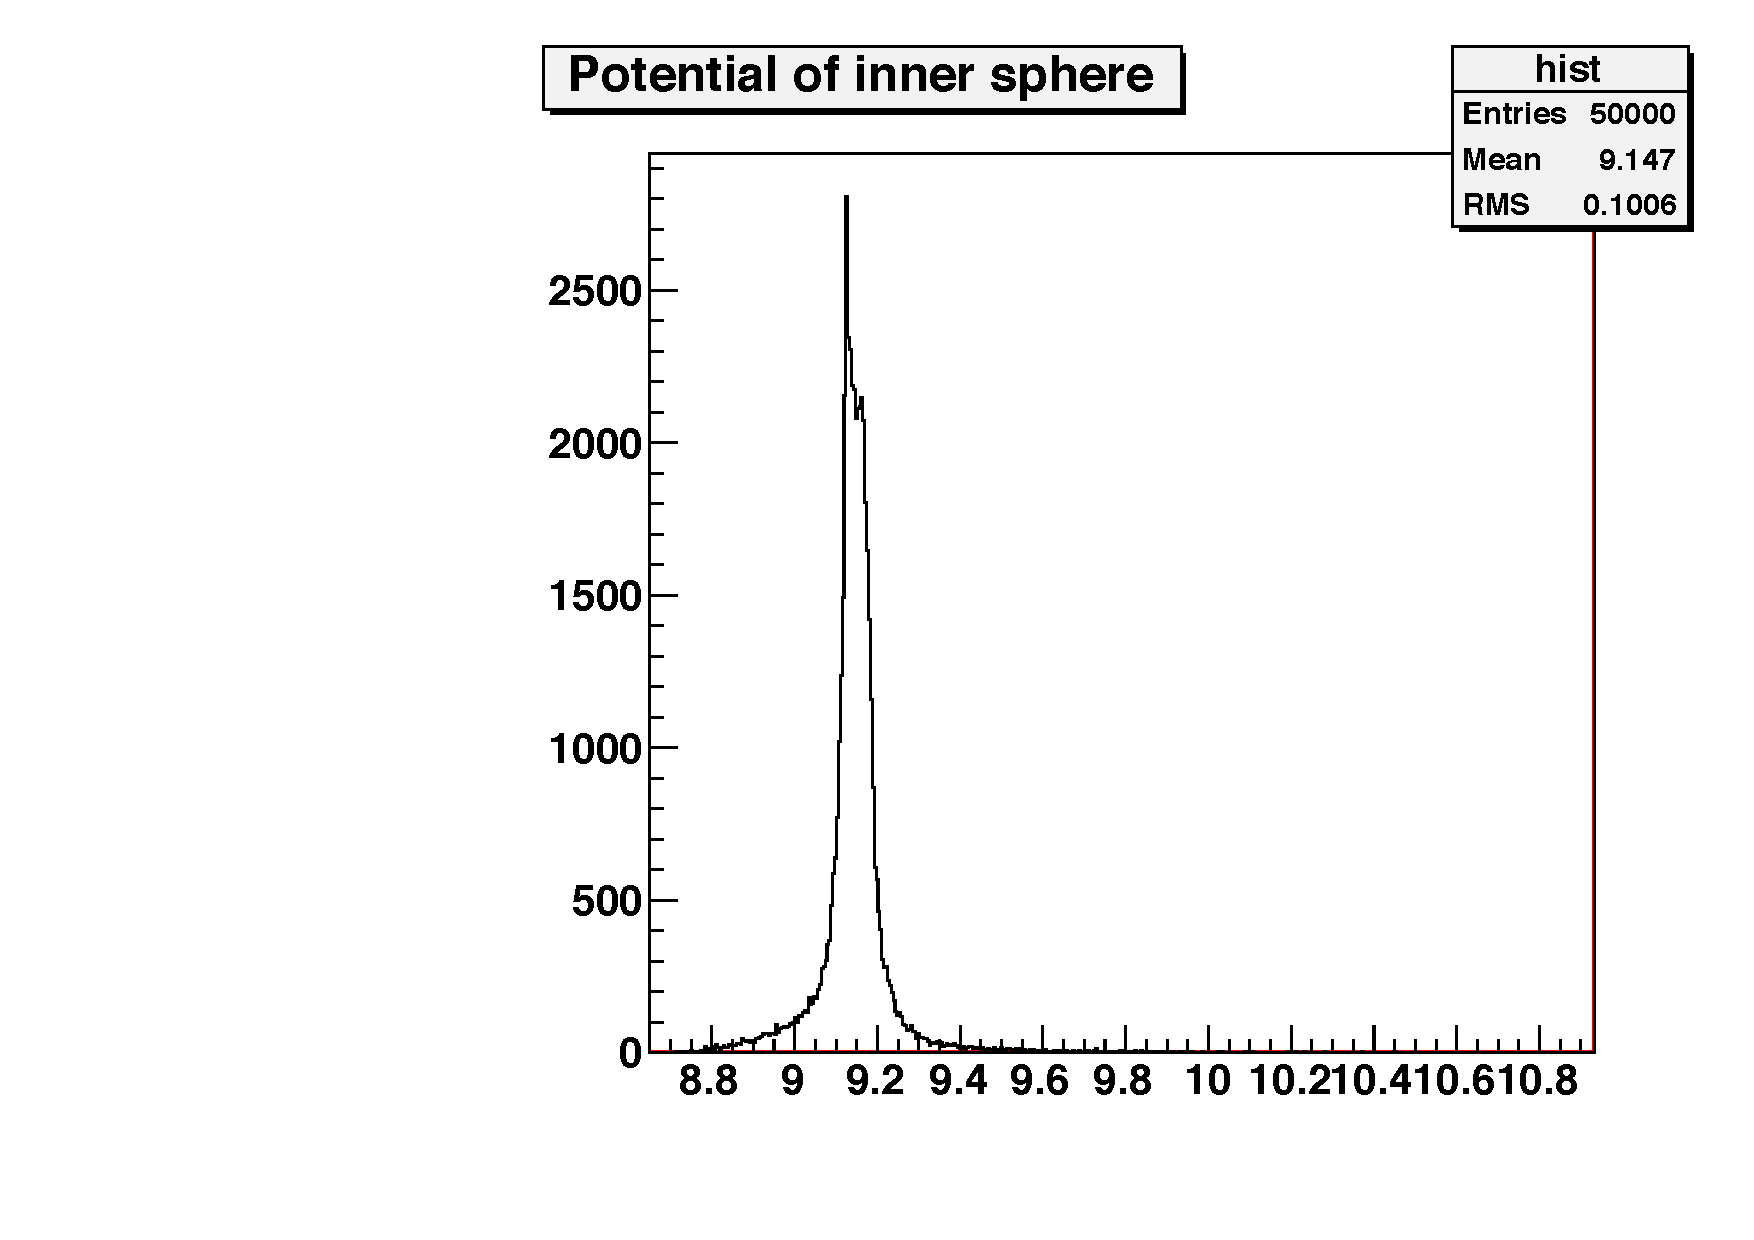
\includegraphics[width=0.5\textwidth]{images/KEMFieldPlots/sphereHist_10e-1.pdf} &
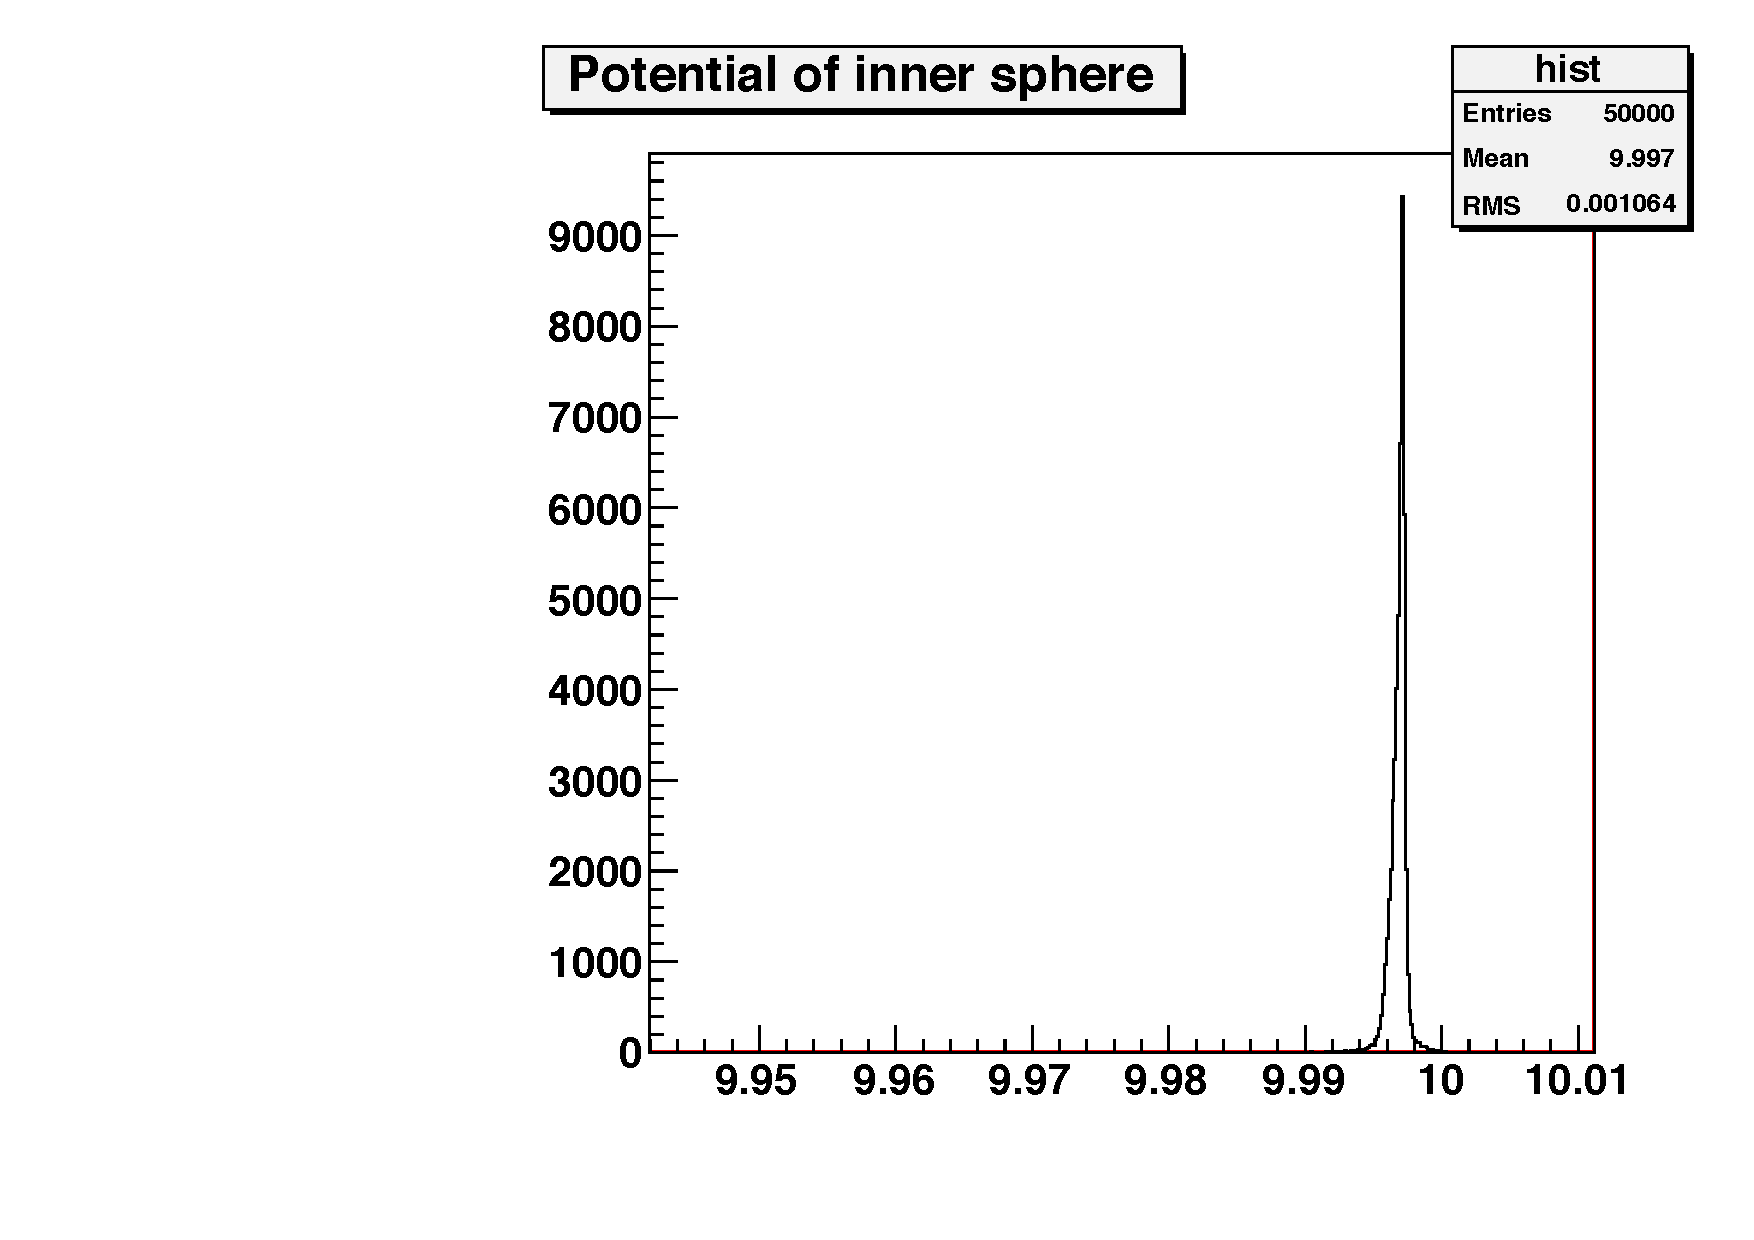
\includegraphics[width=0.5\textwidth]{images/KEMFieldPlots/sphereHist_10e-4.pdf} \\
\end{tabular}
\caption{Potential sampled from inside the smaller nested sphere (at 10 V) for a charge distribution computed from RH with an electrode accuracy requirement of $10^{-1}$ (left) and $10^{-4}$ (right).}
\label{fig:ns_results}
\end{center}
\end{figure}

\subsubsection{Dielectrics}

The Robin Hood method is extremely effective in solving general matrix-inversion equations such as those found in electrostatics, where one effectively solves for the equation...

\begin{equation}
U_i = \sum_{j=1}^N I_{ij} \sigma_j
\end{equation}

\noindent where $U_i$ is the potential of the sub-element $i$, $\sigma_j$ is the charge density of sub-element $j$ of $N$ and $I_{ij}$ is given by...

\begin{equation}
I_{ij} = \frac{1}{4\pi\epsilon_0}\int_{\Delta S_j} \frac{dS_j}{|\vec{r}_i - \vec{r}_j|} 
\end{equation}

The integral expression $I_{ij}$ depends on the distance between point $\vec{r}_i$ and $\vec{r}_j$.  Note that we have implicitly assumed that the surface area $\Delta S_j$ is small enough that the charge distribution within it is constant.

We can expand the Robin Hood method such that it can be used for dielectrics as well.  In the latter case, we need to modify the matrix equation to deal not with potentials (which are fixed at the surface of a conductor) but the boundary conditions imposed by Maxwell's equations~\cite{Rao}.

Therefore, let us take the boundary condition that at the insulator-insulator interface, the displacement vector $\vec{\bf D}$ is continuous across the surface.  This imposes the following condition:

\begin{equation}
\epsilon_i^+ \vec{\bf E}^+_i \cdot \hat{\bf n} - \epsilon_i^- \vec{\bf E}^-_i \cdot \hat{\bf n} = 0
\end{equation} 

\noindent where $\epsilon^{\pm}_i$ is the permittivity above and below the surface of the subelement $i$, $\vec{\bf E}^\pm$ is the electric field, and $\hat{\bf n}$ is the surface normal vector at the insulator-insulator interface at location $i$.  The electric field can be written in integral form as the following...

\begin{equation}
\vec{\bf E}^{\pm}_i = \sum_{j=1}^{N} \frac{\sigma_j}{4\pi\epsilon_0}\int_{\Delta S_j} \frac{(\vec{\bf r}_i - \vec{\bf r}_j)}{|\vec{r}_i - \vec{r}_j|^3} dS_j \pm \hat{\bf n}_i \frac{\sigma_i}{2 \epsilon_0}
\end{equation}

With some manipulation of the above equation, one can re-write the above expression again as a matrix equation.

\begin{equation}
\Psi_i = \sum_{j=1}^{N} \eta_{ij} \sigma_j
\end{equation}

\noindent where for $i\neq j$ we have

\begin{equation}
\eta_{ij} = \frac{1}{4\pi\epsilon_0}\int_{\Delta S_j} \frac{(\vec{\bf r}_i - \vec{\bf r}_j)}{|\vec{r}_i - \vec{r}_j|^3} \cdot \hat{\bf n}_i dS_j
\end{equation}

\noindent and for $i\equiv j$ we have

\begin{equation}
\eta_{ii} = \frac{1}{4\pi\epsilon_0}\frac{2\pi (\epsilon^+_i + \epsilon^-_i)}{\epsilon^+_i - \epsilon^-_i}
\end{equation}

The constraint vector, $\Psi_i$, is simply the null vector.

Formulated in this manner, and taking advantage of the linearity of electric fields, one can impose the same algorithm for solving conductors as one does for insulators.  There exist, however, a few caviats need to be considered.

\begin{enumerate}
\item As this method involves the calculation of the electric field, three components (rather than one) will need to be calculated for each sub-element.
\item This method is well-defined for the case of bound charges from linear media.  For inhomogeneous media, one would need to divide the volume into surfaces and impose the constraint at different depths.
\item Insulators should be treated individually (i.e. no charge exchange between conductors and insulators allowed).
\item Since the system depends on the surface normal $\hat{\bf n}$, one needs to be mindful of the orientation of the surface.
\end{enumerate}

Dielectric media is now implemented in Kassiopeia and has been used in the computation of the fields near the detector region (see Fig.~\ref{fig:detector}).  Preliminary results seem to indicate the method works well.
